\section{1184049 - John Kevin Giraldi}
\subsection{Teori}
\begin{enumerate}

	\item Definisi Kecerdasan Buatan
	\hfill\break
Artificial Intelligence atau kecerdasan buatan adalah sistem komputer yang mampu melakukan tugas-tugas yang biasanya membutuhkan kecerdasan manusia. Jadi secara singkat AI merupakan inovasi yang dibuat manusia untuk menggantikan atau membantu mempermudah pekerjaan manusia yang biasa membutuhkan kecerdasan manusia untuk pengerjaannya menjadi alat/sistem.

	\item Sejarah dan Perkembangan
	\hfill\break
Sejarah kecerdasan buatan diawali pada zaman kuno dan memuncak dalam penemuan komputer digital yang dapat diprogram pada tahun 1940-an, sebuah mesin yang didasarkan pada esensi abstrak penalaran matematika. 
Istilah kecerdasan buatan pada mulanya dikemukakan pada tahun 1956 di Konferensi Darthmouth. Sejak masa itu, kecerdasan buatan terus dikembangkan karena berbagai penelitian mengenai teori-teori dan prinsip-prinsipnya juga terus berkembang. Walaupun istilah kecerdasan buatan baru muncul tahun 1956, tetapi teori-teori yang mengarah ke kecerdasan buatan sudah muncul sejak tahun 1941.
	

	\item Kecerdasan buatan terbagi atas beberapa metode yaitu:
	\hfill\break
	Supervised learning,  Klasifikasi, Regresi,Unsupervised Learning, Dataset, Trainingset dan juga Testingset.
	\begin{itemize}
		\item Supervised Learning
		\hfill\break
Supervised learning (pembelajaran terarah) adalah metode pembelajaran mesin di mana pengguna mengharapkan hasil, dan informasinya diketahui atau dimiliki oleh sistem. Artinya metode pembelajaran bekerja dengan menggunakan kembali masukan atau data pengguna dan hasil keluaran yang sebelumnya diselesaikan oleh sistem. Supervised Learning itu sendiri dapat dibagi lagi menjadi regresi dan klasifikasi.
		\item Klasifikasi
		\hfill\break
Klasifikasi adalah teknik yang digunakan untuk mengklasifikasikan beberapa item yang tidak berlabel ke dalam satu set kelas diskrit. Klasifikasi mencoba mempelajari hubungan antara sekumpulan variabel fitur dan variabel target. Dalam klasifikasi, variabel targetnya adalah tipe kategori.
		\item Regresi
		\hfill\break
Regresi adalah teknik analisis yang digunakan untuk mengidentifikasi hubungan antara dua variabel atau lebih. Tujuan dari regresi adalah untuk menemukan fungsi yang memodelkan data dengan meminimalkan kesalahan atau perbedaan antara nilai prediksi dan nilai sebenarnya.
		\item Unsupervised Learning 
		\hfill\break
Unsupervised Learning adalah metode lain dalam materi pembelajaran mesin, di mana tidak ada yang bisa mengetahui hasil yang diharapkan. Tujuan utama dari metode pembelajaran ini adalah agar para penggunanya dapat mengelompokkan objek-objek yang dianggap serupa pada suatu ruang atau area tertentu.
Kumpulan data adalah objek yang mirip dengan kamus, yang menyimpan semua data dan beberapa metadata tentang data.
		\item Data set
		\hfill\break
Data set	merupakan kondisi dimana hanya terdapat inputan data tanpa memiliki viariasi output yang sesuai
		\item Training Set
		\hfill\break
Training Set adalah bagian dari Data Set yang dilatih untuk membuat prediksi atau menjalankan fungsi algoritma ML. Dengan memberikan petunjuk melalui algoritma sehingga mesin yang dilatih dapat menemukan korelasinya sendiri atau mempelajari pola dari data yang diberikan. Testing Set adalah bagian dari data set yang diuji untuk melihat akurasinya, atau dengan kata lain, untuk melihat performanya.		
		\item Testing Set
		\hfill\break
Testing Set	merupakan bagian data set yang digunakan untuk pengujian dari properti yang dipelajari
	\end{itemize}
\end{enumerate}
\subsection{Praktek}
\begin{enumerate}
	\item Instalasi Library scikit dari Anaconda, mencoba kompilasi dan uji coba ambil contoh kode dan lihat variabel explorer
	\hfill\break
	\begin{figure}[h]
		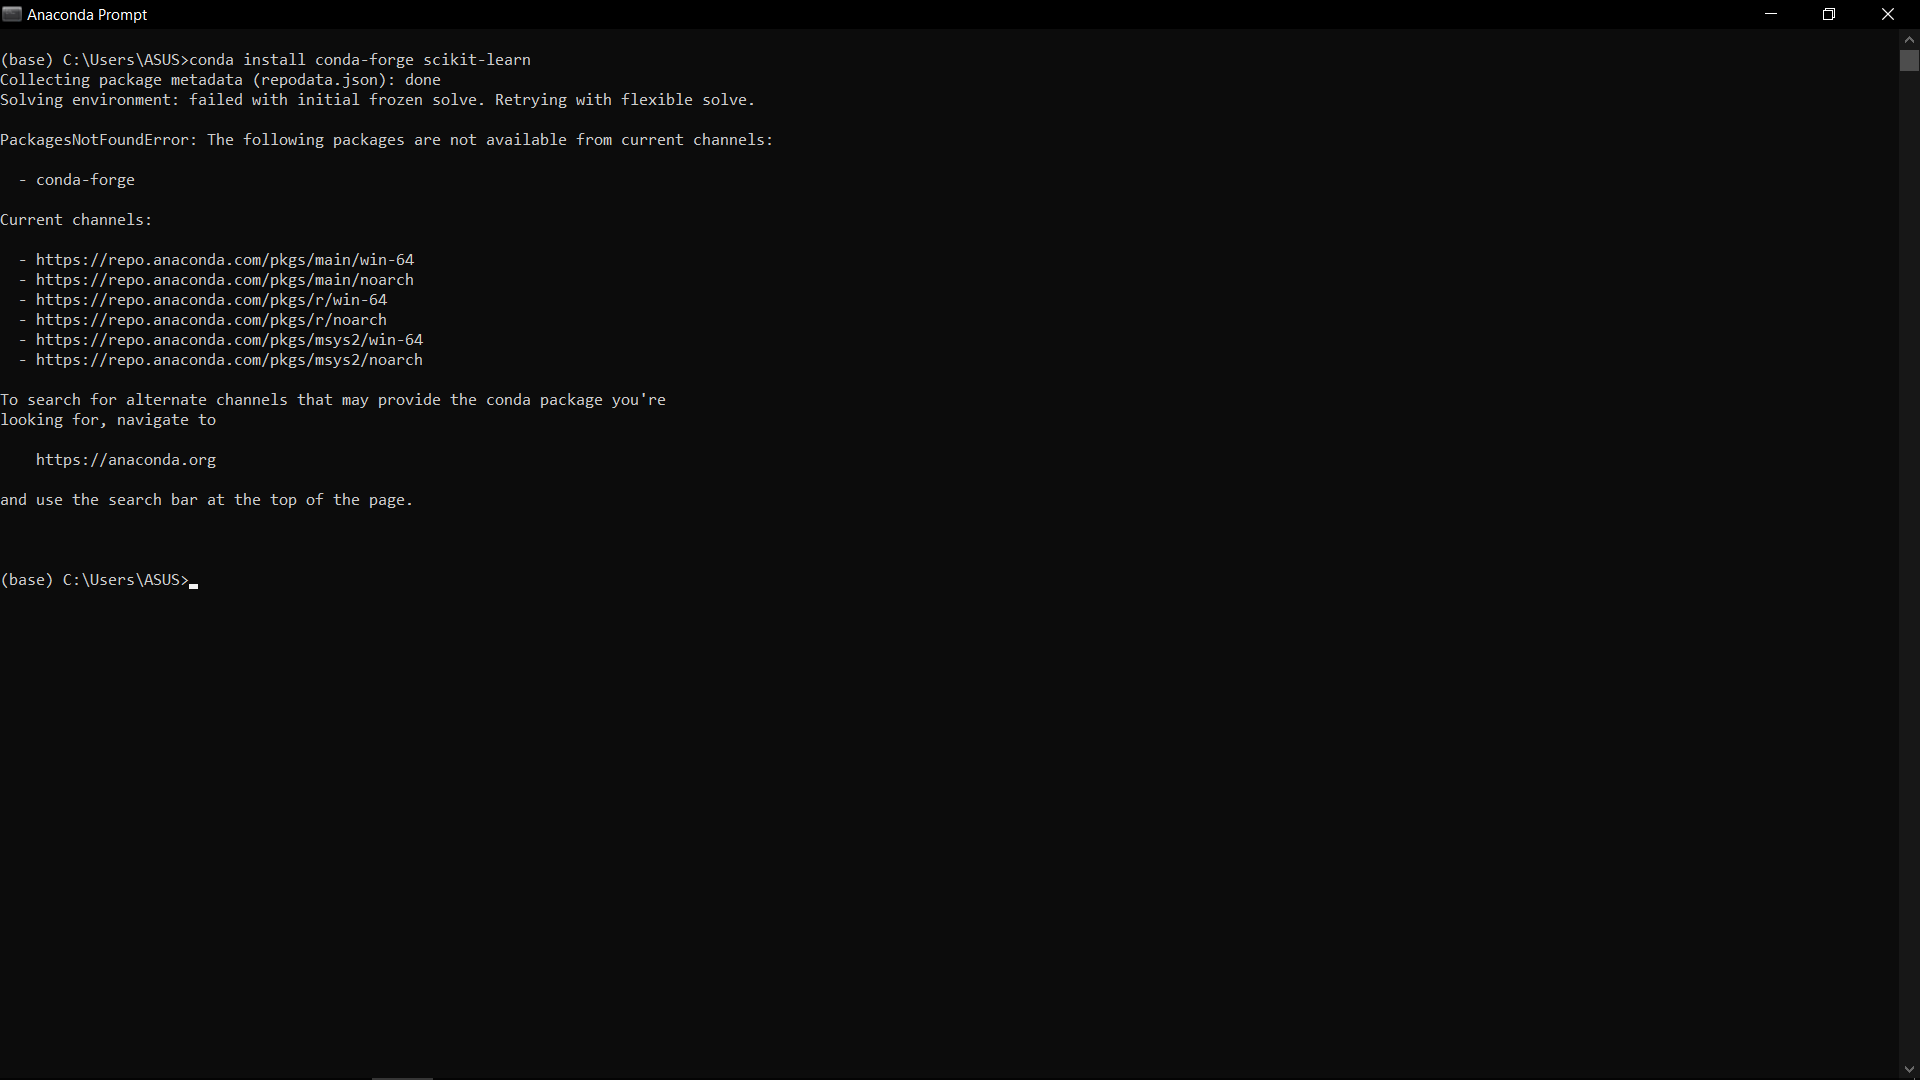
\includegraphics[width=10cm]{figures/1184049/1.png}
		\centering
		\caption{Instalasi Library Scikit Learn}
	\end{figure}
	\begin{figure}[h]
		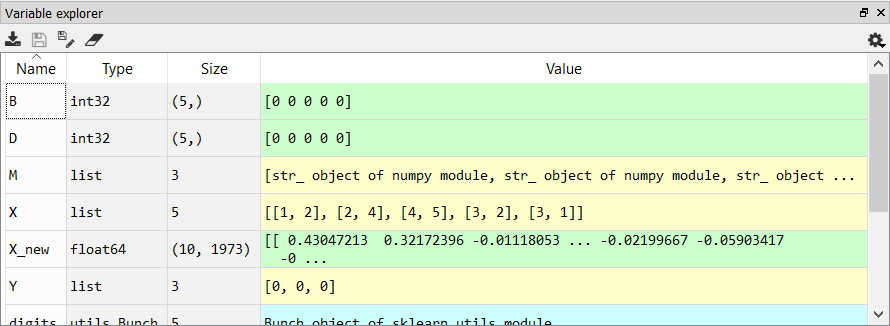
\includegraphics[width=10cm]{figures/1184049/VAR.png}
		\centering
		\caption{Isi Variabel Explorer}
	\end{figure}
	\newpage\item Uji coba loading an example dataset
	\hfill\break
\lstinputlisting[firstline=7, lastline=16]{src/1184049/1184049.py}
\item Uji coba Learning dan predicting
	\hfill\break
	\lstinputlisting[firstline=27, lastline=37]{src/1184049/1184049.py}
\item Uji coba Model Persistence
	\hfill\break
	\lstinputlisting[firstline=56, lastline=107]{src/1184049/1184049.py}
	\item Uji coba Conventions
	\hfill\break
	\lstinputlisting[firstline=42, lastline=53]{src/1184049/1184049.py}
	\end{enumerate}
	\subsection{Penanganan Error}
\begin{enumerate}
	\item ScreenShoot Error
	\begin{figure}[h]
		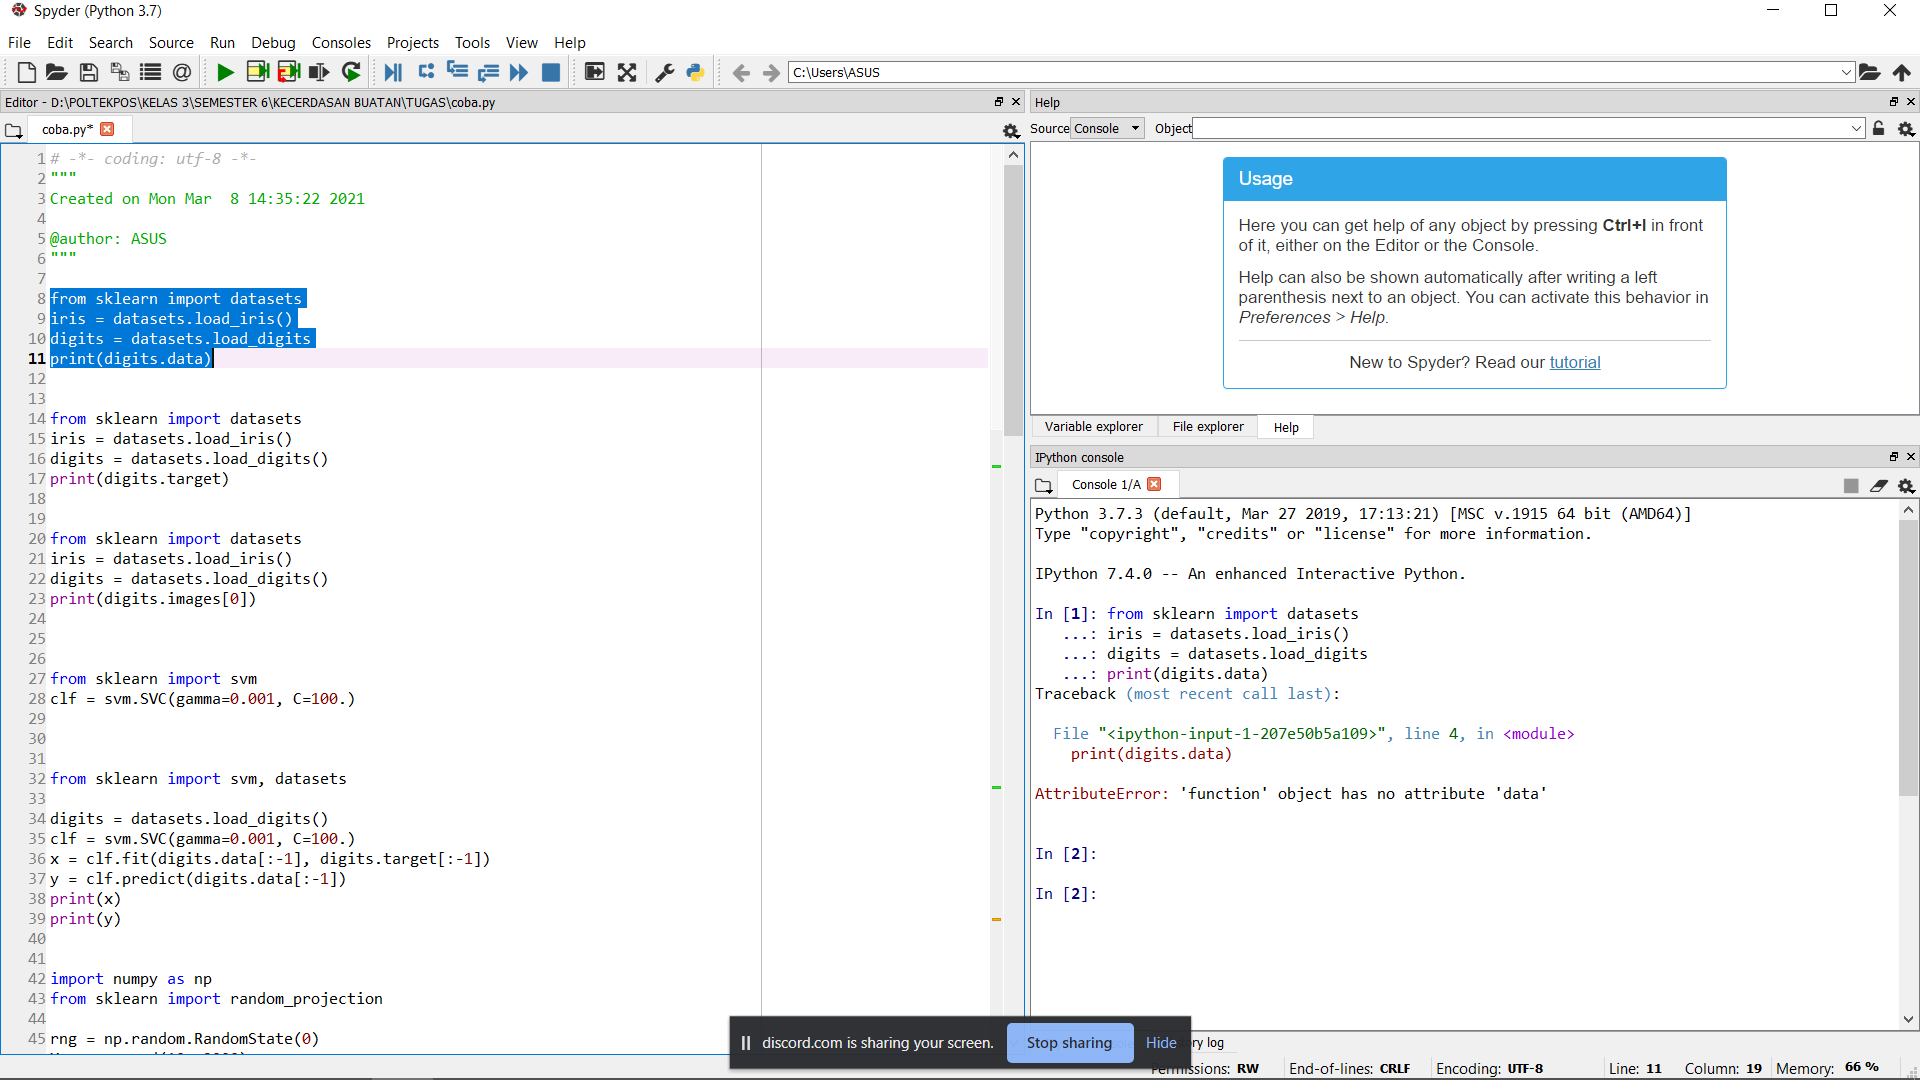
\includegraphics[width=10cm]{figures/1184049/EROR1.png}
		\centering
		\caption{Not Defined Syntax}
	\end{figure}
	\item Cara Penangan Error
\hfill\break Tambahkan variabel yang kurang pada kode program agar dapat terbaca
	\end{enumerate}
	\subsection{Bukti Tidak Plagiat}
\begin{figure}[h]
	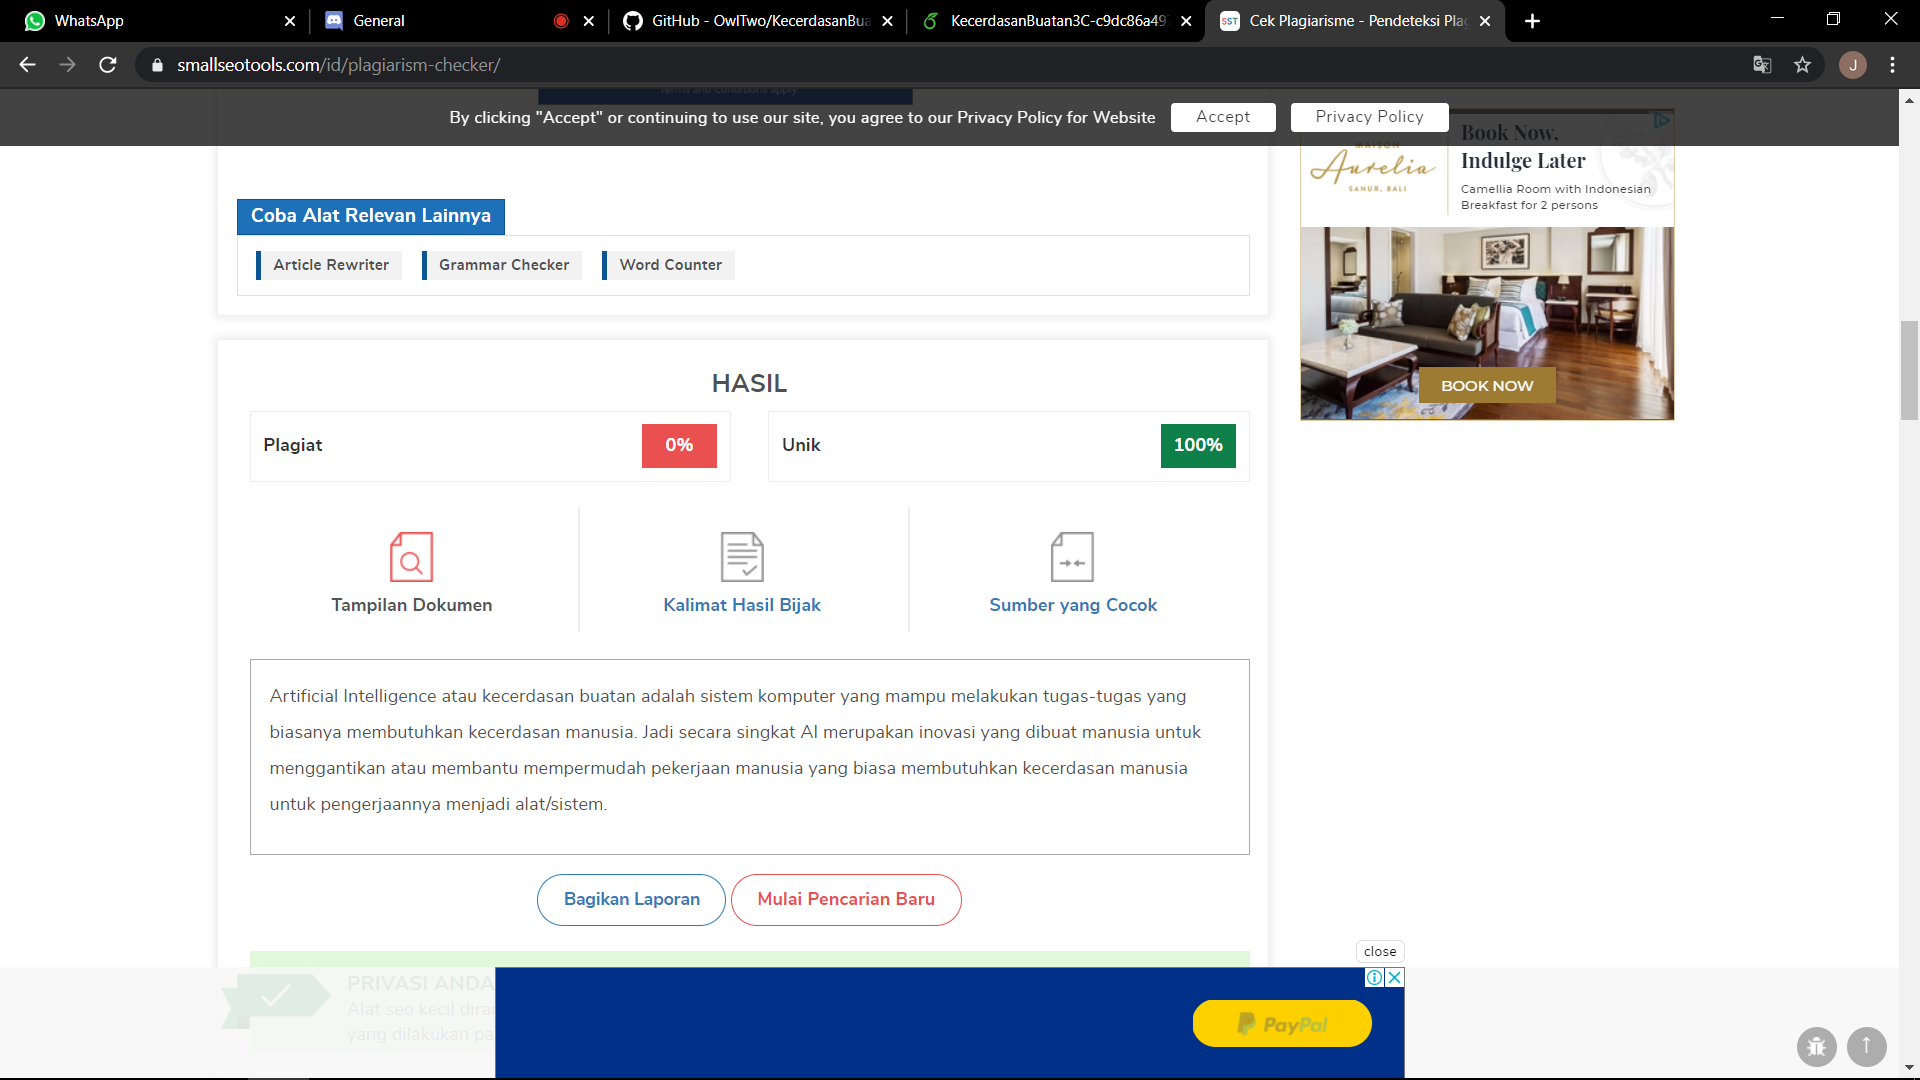
\includegraphics[width=10cm]{figures/1184049/PL1.png}
	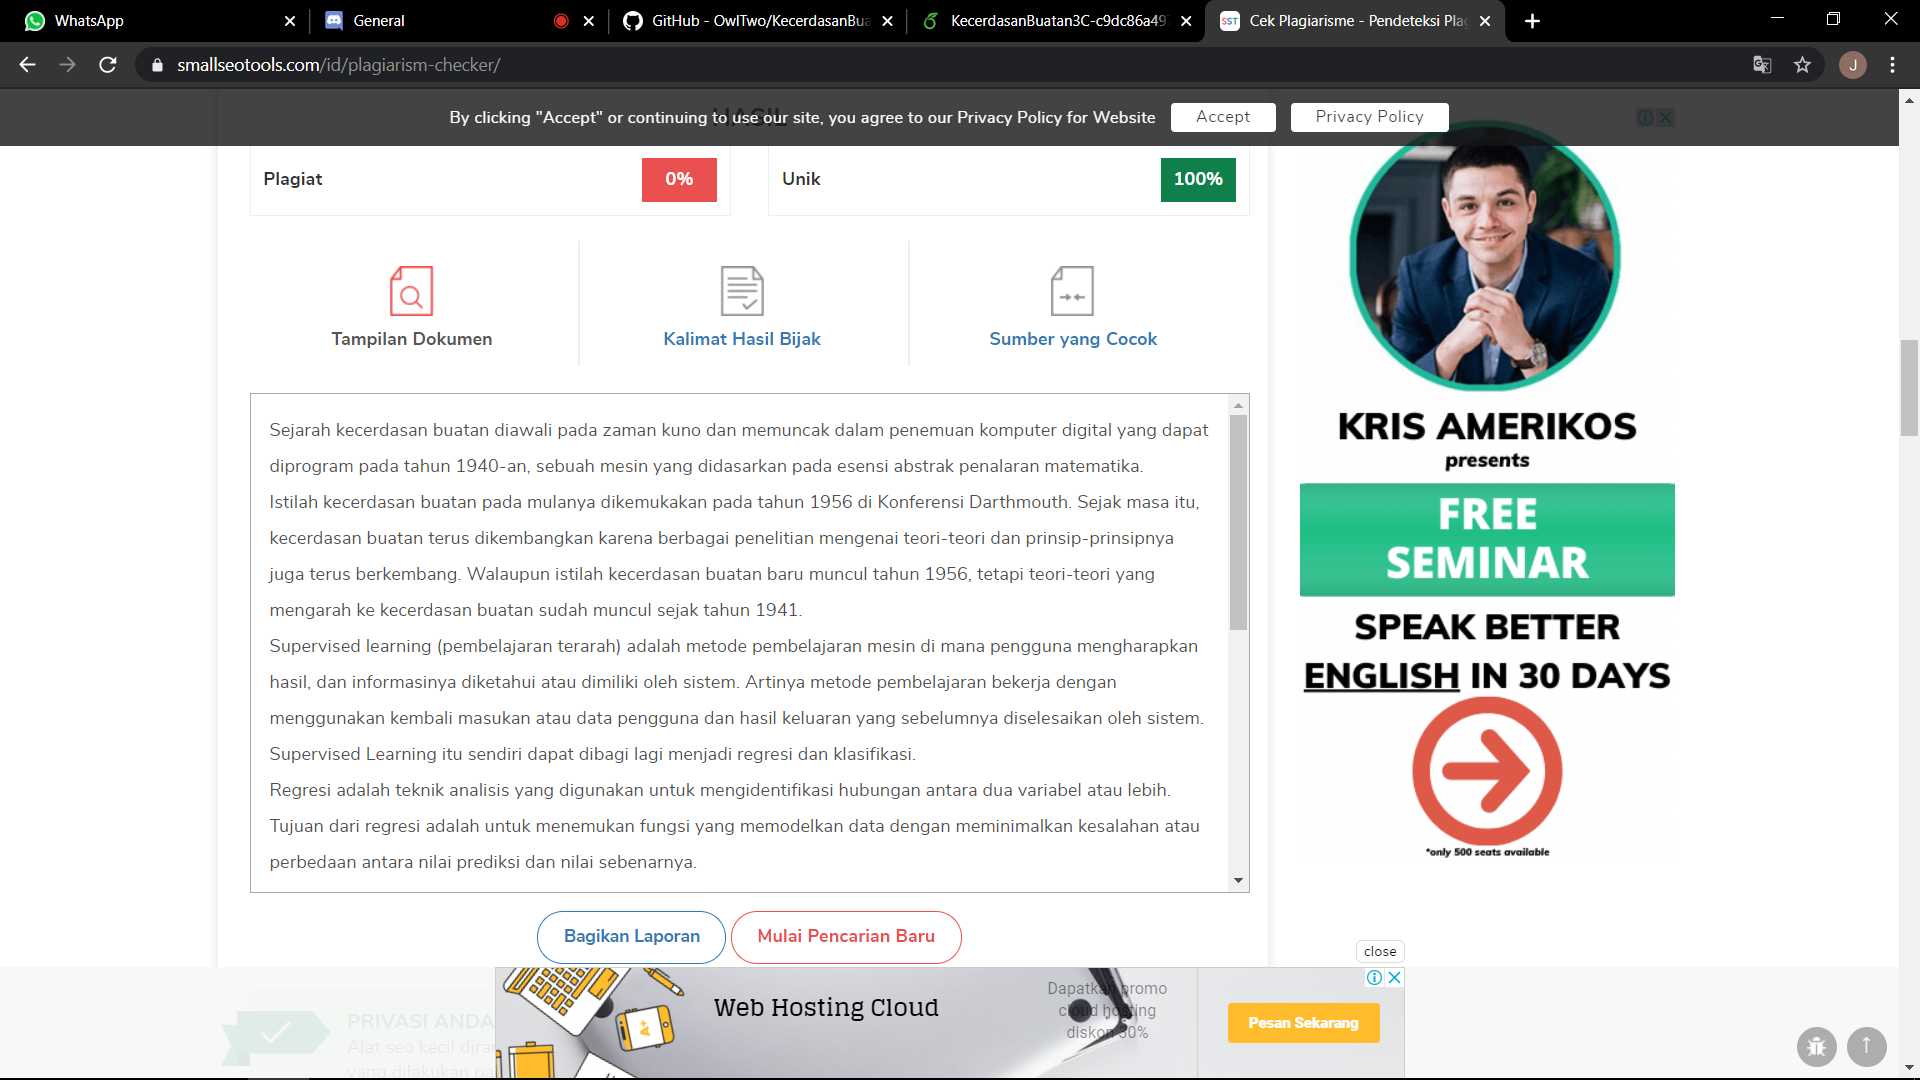
\includegraphics[width=10cm]{figures/1184049/PL2.png}
	\centering
	\caption{Bukti Tidak Melakukan Plagiat Chapter 1}
\end{figure}